\subsection{RISC-V硬件架构}\label{riscv}

通用CPU一般能够在硬件上支持内存空间的隔离,使得多个程序在各自独立的内存空间中并发执行。这种硬件机制即支持用户特权级和内核特权级。应用程序运行在用户特权级,这样应用不能执行特权指令,且不能破坏操作系统内核的数据和操作系统执行过程。而操作系统内核运行在内核特权级,可以访问特权指令,并管理和控制应用程序,硬件外设等。所以对于操作系统而言,需要CPU硬件至少支持用户特权级和内核特权级(控制隔离),以及内存空间隔离(数据隔离)。

RISC-V是发源于Berkeley的开源instruction set architecture
(ISA)。在继续阅读前,对RISCV指令集和架构特别感兴趣的同学可仔细阅读RISC-V的Specifications。当前用户态指令集规范的版本为2.2,特权态指令集规范的版本为1.10。

\begin{itemize}
\item
  \href{https://riscv.org/specifications/}{User-Level ISA Specification
  v2.2}
\item
  \href{https://riscv.org/specifications/privileged-isa}{Draft
  Privileged ISA Specification v1.10}
\end{itemize}

\subsection{Modular ISA}\label{modular-isa}

RISC-V ISA是模块化的,它由一个基本指令集和一些扩展指令集组成

\begin{itemize}
\item
  Base integer ISAs

  \begin{itemize}
  \item
    RV32I
  \item
    RV64I
  \item
    RV128I
  \end{itemize}
\item
  Standard extensions

  \begin{itemize}
  \item
    M: Integer \textbf{M}ultiply
  \item
    A: \textbf{A}tomic Memory Operations
  \item
    F: Single-percison \textbf{F}loating-point
  \item
    D: \textbf{D}ouble-precision Floating-point
  \item
    G: IMAFD, \textbf{G}eneral Purpose ISA
  \end{itemize}
\end{itemize}

举例来说,\texttt{RV32IMA}表示支持基本整数操作和原子操作的32位RISC-V指令集。对于一般在用户态执行的应用程序,只需要上述用户态指令集就基本足够了。但如果是象操作系统这样的软件,需要控制整个计算机硬件,则只使用用户态指令集是不够的,还需要在处于内核特权级的CPU状态下执行特权指令集。

\subsection{Privileged ISA}\label{privileged-isa}

\subsubsection{Software Stacks}\label{software-stacks}

RISC-V在设计时就考虑了硬件虚拟化的需求,三种典型RISC-V系统的结构如下

%\begin{figure}[htbp]
%\centering
%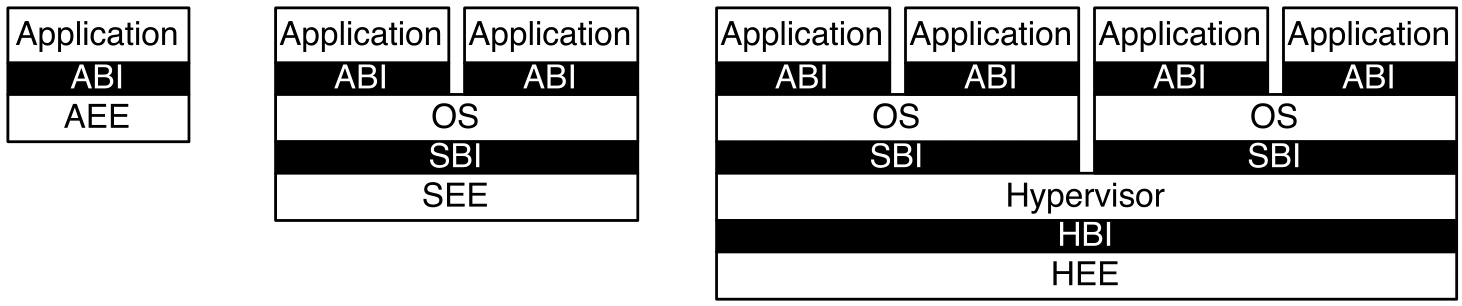
\includegraphics{figures/software-stacks.png}
%\caption{software-stacks}
%\end{figure}

上图中各个英文缩写对应的全称如下

\begin{itemize}
\item
  ABI: Application Binary Interface
\item
  AEE: Application Execution Environment
\item
  SBI: Supervisor Binary Interface
\item
  SEE: Supervisor Execution Environment
\item
  HBI: Hypervisor Binary Interface
\item
  HEE: Hypervisor Execution Environment
\end{itemize}

RISC-V通过各层之间的Binary
Interface实现了对下一层的抽象,方便了虚拟机的实现以及OS在不同RISC-V架构间的移植。采用了图中第二种结构,\href{https://github.com/riscv/riscv-pk}{bbl}在其中充当了SEE的角色。

\subsubsection{Privilege Levels}\label{privilege-levels}

RISC-V共有4种不同的特权级,与x86不同的是,RISC-V中特权级对应数字越小,权限越低

\begin{longtable}[c]{@{}cccc@{}}
\toprule
Level & Encoding & Name & Abbreviation\tabularnewline
\midrule
\endhead
0 & 00 & User/Application & U\tabularnewline
1 & 01 & Supervisor & S\tabularnewline
2 & 10 & Hypervisor & H\tabularnewline
3 & 11 & Machine & M\tabularnewline
\bottomrule
\end{longtable}

一个RISC-V的实现并不要求同时支持这四种特权级,可接受的特权级组合如下

\begin{longtable}[c]{@{}cll@{}}
\toprule
Number of levels & Supported Modes & Intended Usage\tabularnewline
\midrule
\endhead
1 & M & Simple embedded systems\tabularnewline
2 & M, U & Secure embedded systems\tabularnewline
3 & M, S, U & Systems running Unix-like operating systems\tabularnewline
4 & M, H, S, U & Systems running Type-1 hypervisors\tabularnewline
\bottomrule
\end{longtable}

目前官方的\href{https://github.com/riscv/riscv-isa-sim}{Spike}模拟器只部分实现了3个特权级。

\subsubsection{Control and Status
Registers}\label{control-and-status-registers}

RISC-V中各个特权级都有单独的Control and Status Registers
(CSRs),其中应当注意的有以下几个

\begin{longtable}[c]{@{}ll@{}}
\toprule
Name & Description\tabularnewline
\midrule
\endhead
sstatus & Supervisor status register\tabularnewline
sie & Supervisor interrupt-enable register\tabularnewline
stvec & Supervisor trap handler base address\tabularnewline
sscratch & Scratch register for supervisor trap handlers\tabularnewline
sepc & Supervisor exception program counter\tabularnewline
scause & Supervisor trap cause\tabularnewline
sbadaddr & Supervisor bad address\tabularnewline
sip & Supervisor interrupt pending\tabularnewline
sptbr & Page-table base register\tabularnewline
mstatus & Machine status register\tabularnewline
medeleg & Machine exception delegation register\tabularnewline
mideleg & Machine interrupt delegation register\tabularnewline
mie & Machine interrupt-enable register\tabularnewline
mtvec & Machine trap-handler base address\tabularnewline
mscratch & Scratch register for machine trap handlers\tabularnewline
mepc & Machine exception program counter\tabularnewline
mcause & Machine trap cause\tabularnewline
mbadaddr & Machine bad address\tabularnewline
mip & Machine interrupt pending\tabularnewline
\bottomrule
\end{longtable}

在继续阅读前,读者应当查阅\href{https://riscv.org/specifications/privileged-isa}{Privileged
Spec 1.9.1}以熟悉以上CSR的功能和用途。

\paragraph{CSR Instructions}\label{csr-instructions}

RISC-V
ISA中提供了一些修改CSR的原子操作,下面介绍之后常用到的\texttt{csrrw}指令

\begin{lstlisting}[language={C}]
# Atomic Read & Write Bit
cssrw rd, csr, rs
\end{lstlisting}

语义上等价的C++函数如下

\begin{lstlisting}[language={C}]
void cssrw(unsigned int& rd, unsigned int& csr, unsigned int& rs) {
   unsigned int tmp = rs;
   rd = csr;
   csr = tmp;
}
\end{lstlisting}

几种有趣的用法如下

\begin{lstlisting}[language={C}]
# csr = rs
cssrw x0, csr, rs

# csr = 0
cssrw x0, csr, x0

# rd = csr, csr = 0
cssrw rd, csr, x0

# swap rd and csr
cssrw rd, csr, rd
\end{lstlisting}
